% --- IMPLEMENTATION AND EXPERIMENTAL SETUP ---

\noindent This chapter describes the Java implementation architecture and the experimental setup used to evaluate the proposed algorithm.

\section{Java Architecture}

The entire system was implemented in Java (JDK 8+) using a modular pipeline architecture across 14 classes and approximately 2,500 lines of code. Each phase of computation is a separate, self-contained class, and data flows through the pipeline via a central data transfer object (SimulationData). Figure~\ref{fig:pipeline_arch} shows the overall architecture.

\begin{figure}[htbp]
\centering
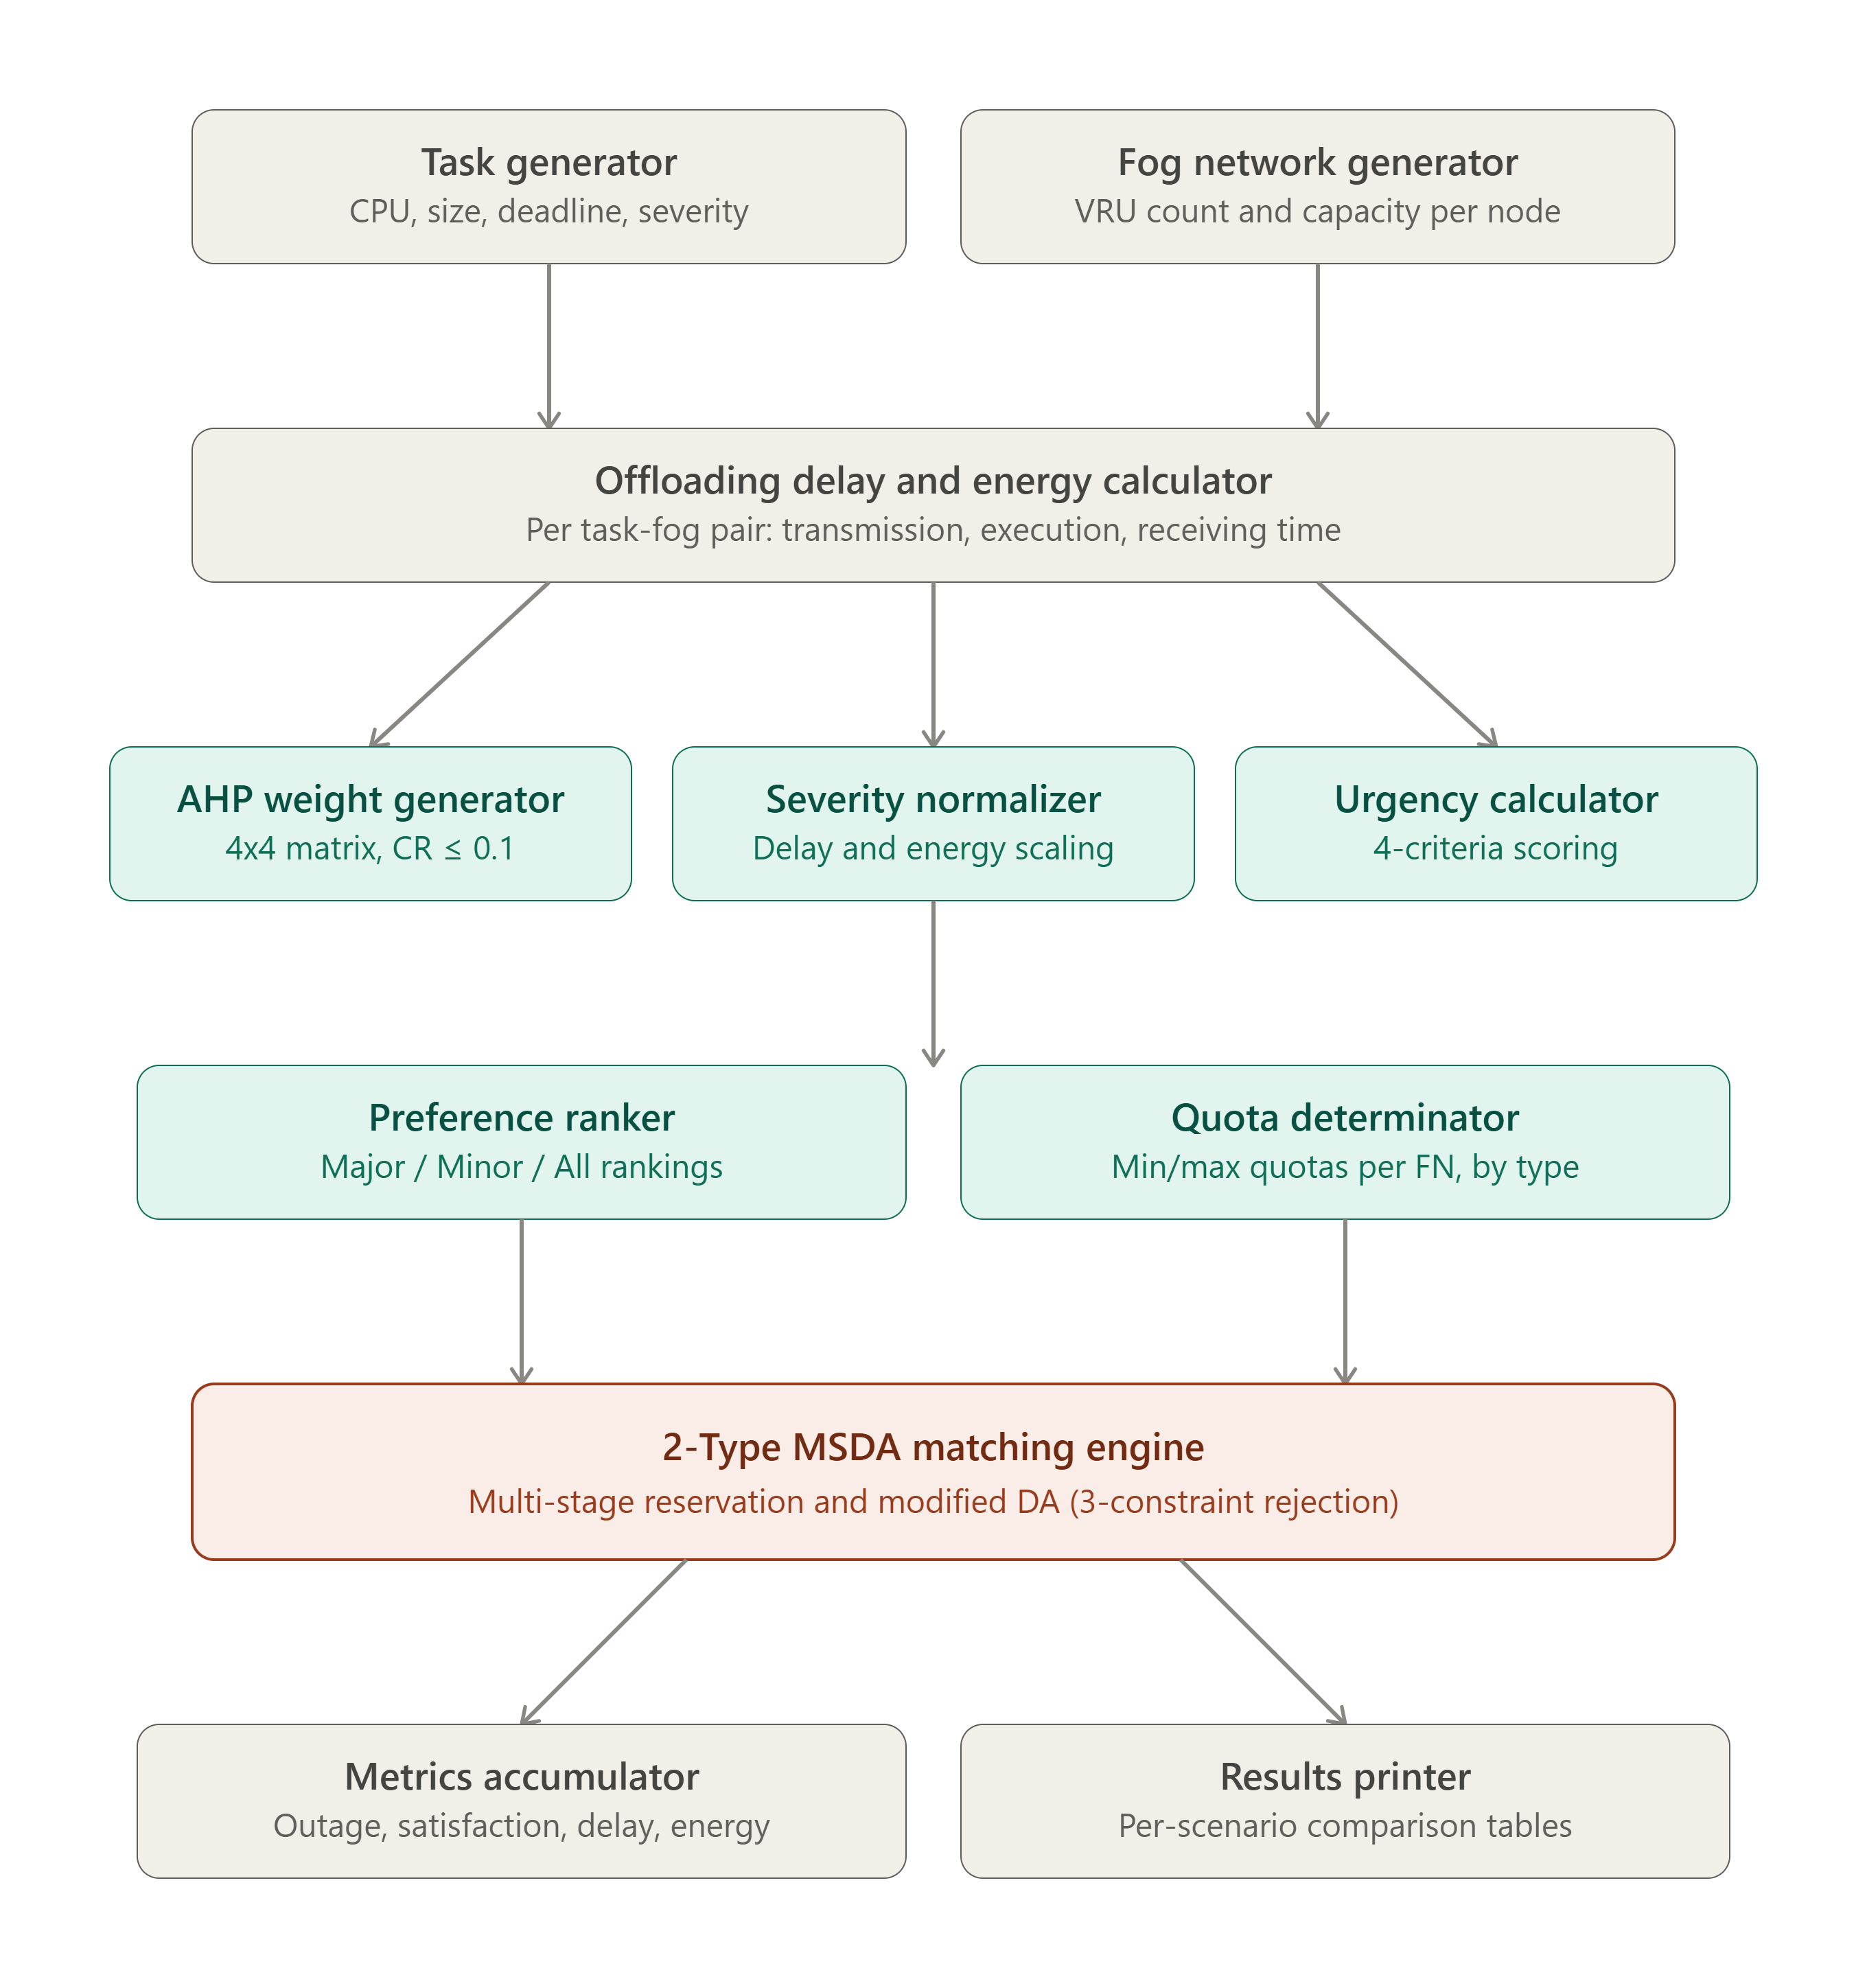
\includegraphics[width=0.95\textwidth]{Images/proposed_2type_msda_pipeline_architecture.png}
\caption{Modular pipeline architecture of the Java implementation showing the 14 classes and data flow.}
\label{fig:pipeline_arch}
\end{figure}

\begin{table}[htbp]
\centering
\begin{tabular}{|l|l|l|}
\hline
\textbf{Category} & \textbf{File} & \textbf{Responsibility} \\
\hline
Orchestrator & Main.java & Entry point; runs full pipeline across scenarios \\
\hline
\multirow{4}{*}{Data Models} & Task.java & Task attributes and per-fog metric arrays \\
 & FogNetwork.java & FN attributes, capacity, and quota fields \\
 & SimulationData.java & DTO bundling all computed arrays \\
 & SimulationConfig.java & Central constants and parameter ranges \\
\hline
\multirow{2}{*}{Generators} & TaskGenerator.java & Random IoT task generation \\
 & FogNetworkGenerator.java & Random fog node generation \\
\hline
\multirow{4}{*}{Calculators} & OffloadingCalculator.java & Delay and energy computation \\
 & Normalizer.java & Min-Max + severity-weight normalisation \\
 & UrgencyCalculator.java & Multi-criteria urgency scoring \\
 & QuotaDeterminator.java & Min/max quota computation \\
\hline
\multirow{2}{*}{Ranking \& Matching} & WeightGenerator.java & AHP 4$\times$4 with CR $\leq$ 0.1 \\
 & PreferenceRanker.java & Fog-side rankings and precedence lists \\
\hline
Matching & MSDAlgorithm.java & Single-Type MSDA, 2-Type MSDA, GPM \\
\hline
\multirow{2}{*}{Output} & SimulationPrinter.java & Results, tables, and utilisation bars \\
 & SimulationMetrics.java & Accumulator for averaging across iterations \\
\hline
\end{tabular}
\caption{File structure and responsibilities of the 14-class Java implementation.}
\label{tab:file_structure}
\end{table}

A critical design decision was the use of deep copy to ensure data independence between algorithm pipelines. All three algorithms (GPM, Baseline, Proposed) start from identical raw data (same fog nodes, same tasks, same delays, same energies). The deep copy creates independent copies so each algorithm modifies its own data without contaminating the others, guaranteeing a fair apples-to-apples comparison.

\section{Experimental Setup}

\subsection{Algorithms Compared}

Three algorithms are evaluated and compared:
\begin{enumerate}
\item \textbf{Greedy Placement Method (GPM)}: Assigns tasks greedily to fog nodes sorted by capacity, with no fairness or urgency considerations. Provides a lower-bound comparison.
\item \textbf{Baseline (M-DAFTO)}: Single-Type MSDA with 2-criteria urgency, 2$\times$2 AHP, and delay-only normalisation \cite{swain2024mdafto}.
\item \textbf{Proposed System (Adapted 2-Type MSDA)}: Severity-aware 2-Type MSDA with 4-criteria urgency, 4$\times$4 AHP, severity-weighted normalisation, and separate Major/Minor quota tracking.
\end{enumerate}

\subsection{Simulation Parameters}

\begin{table}[htbp]
\centering
\begin{tabular}{|l|l|}
\hline
\textbf{Parameter} & \textbf{Range / Value} \\
\hline
Number of tasks & 250, 500, 1000, 2000 (per scenario) \\
Number of fog nodes & 5 \\
CPU demand & [210.0, 480.0] Mcycles \\
Input size & [300.0, 600.0] KB \\
Output size & [10.0, 20.0] KB \\
Deadline & [15.0, 22.0] seconds \\
Fog CPU capacity & [6.0, 10.0] GHz \\
Fog VRU count & [200, 500] \\
Phase & ``Pre-Surgery'' / ``Post-Surgery'' \\
Severity & ``Minor'' / ``Major'' (50/50) \\
Uplink data rate & 2500 KB/s (20 MHz) \\
Downlink data rate & 2500 KB/s (20 MHz) \\
Transmission power & 0.5 W \\
Execution power & 1.0 W \\
Receiving power & 0.5 W \\
\hline
\end{tabular}
\caption{Simulation parameters and their ranges, adapted from \cite{swain2024mdafto}.}
\label{tab:sim_params}
\end{table}

The experimental setup follows standard fog computing evaluation practice \cite{gupta2017ifogsim}. Four task scales (250, 500, 1000, 2000) represent increasing load levels from normal operation to extreme overload. Each scenario uses 5 randomly generated fog nodes. Results are averaged over 10 independent iterations to smooth out randomness, giving a total of $4 \times 10 \times 3 = 120$ algorithm runs.

\subsection{Metrics}

The following metrics were measured for each algorithm run:
\begin{itemize}
\item Overall outage probability (\%)
\item Major task outage probability (\%)
\item Minor task outage probability (\%)
\item Total and average offloading delay (seconds)
\item Total energy consumed (Joules)
\item Task satisfaction (\%) --- measures how close each task's assignment is to its most preferred fog node
\item FN satisfaction (\%) --- measures how well each fog node's assigned tasks match its preference ranking
\end{itemize}